\documentclass{article}

\title{neotoma: A Programmatic Interface to the Neotoma Paleoecological Database}
\author{Simon Goring}

\usepackage{Sweave}
\begin{document}
\Sconcordance{concordance:neotoma_sweave.tex:neotoma_sweave.Rnw:%
1 5 1 1 0 26 1 1 2 1 0 6 1 1 2 6 0 1 2 3 1 1 4 7 0 1 3 4 1 1 3 1 0 1 7 %
9 0 1 3 3 1 1 5 8 0 1 3 15 1 1 3 5 0 1 3 4 1 1 3 2 0 1 2 1 1 1 2 1 8 10 %
0 1 3 4 1 1 19 17 0 1 4 2 0 1 5 3 0 1 5 3 0 2 2 1 8 6 0 1 3 1 0 1 2 5 0 %
1 3 3 1}

\maketitle

\section*{Abstract}

Paleoecological data is an integral part of ecological analysis.  It provides an opportunity to study vegetation and climate interactions at time scales that cannot be observed through modern field studies, and allows us to observe changes in so-called 'slow' processes associated with centennial and millennial scale changes in climate.
Here we describe the R package \texttt{neotoma}, to be used to obtain and manipulate paleoecological data from the Neotoma Paleoecological Database.  \texttt{neotoma} searches the Neotoma Database for datasets associated with location, taxa or dataset types using the database's Application Programming Interface.  The package can return full datasets or metadata associated with sites and provides the ability to standardize taxonomies using one of several recognized standard taxonomies from the published literature.
To assist with the use of the package we provide examples of key functions using examples from the published literature, for both plant and mammal taxa.

\section*{Introduction}
Paleoecological data is increasingly used to understand patterns of biogeographical, climatic and evolutionary change at multiple spatial and temporal scales.  Paleoecoinformatics (\cite{brewer2012paleo}) is increasingly providing tools to researchers across disciplines to access and use large datasets spanning thousands of years.  These datasets may be used to provide better insight into patterns of biomass burning (Blarquez et al, 2013; Power et al), regional vegetation change (Blois et al., 2012) or changes in physical processes over time (\cite{goring2012depo}).  The statistical software R (\cite{RCoreTeam2014}) is commonly used for analysis of paleoecological data and several packages in R exist for analysis (analogue: \cite{analogue2013, analogue2007}; rioja: \cite{rioja2013}, Bchron: \cite{bchron2014}, paleofire: \cite{paleofire2014}). Notwithstanding, the use of extensive paleoecological resources within R has traditionally relied on \emph{ad hoc} methods of obtaining and importing data.  This has meant reliance on static online datasets such as the NOAA Paleoclimate repository or North American Modern Pollen Database, and on the distribution of individual datasets from author to analyst.

With an increasing push to provide paleoecological publications that include numerically reproducible results (e.g., \cite{goring2012depo,gill2013linking,goring2013pollen}) it is important to provide tools that allow analysts to directly access dynamic datasets, and to provide tools to support reproducible workflows.  The \texttt{ropensci} project has provided a number of tools that can directly interact with Application Programmatic Interfaces (APIs) to access data from a number of databases including rfishbase (FishBase: \cite{boettiger2012rfishbase}) and taxize (Encyclopedia of Life, iPlant/Taxosaurus and others: \cite{chamberlain2013taxize}) among others.

To illustrate use cases for the \texttt{neotoma} package we present examples drawn from the paleoecological literature to illustrate how \texttt{neotoma} provides the tools to perform research that is critical to understanding paleoecological change in the Pleistocene in an open and reproducible manner.

\section*{The \texttt{neotoma} package}

Here we describe \texttt{neotoma}, an R package that acts as an interface between a large dynamic database (the Neotoma Paleoecological Database; http://neotomadb.org) and statistical tools in R.  The \texttt{neotoma} package uses a programmatic interface (an API) to send data requests to Neotoma, and then forms data objects that can interact with existing packages such as \texttt{analogue} and \texttt{rioja}.  The \texttt{neotoma} package also includes tools to standardize pollen data across sample sites using a set of commonly accepted pollen taxa.

\section*{Examples}
\subsection*{\emph{Pinus} Migration}
Macdonald and Cwynar (1985) used pollen percentage data for Pinus to map the northward migration of lodgepole pine (Pinus contorta) following glaciation.  In their study a cutoff of 15\% Pinus pollen is associated with presence at pollen sample sites.  Recent work by Strong and Hills (2013) has remapped the migration front using a lower pollen proportion (5\%) and more sites.  Here we attempt to replicate the analysis as an example both of the strengths of the package and limitations of paleoinformatic approaches.

To begin we must define a spatial bounding box and a set of taxa of interest.  Strong and Hills (2013) use a region approximately bounded by 54oN to the south and 65oN to the North, and from 110oW to 130oW.  The command \texttt{get\_site} is used to find all sites within a bounding box:

\begin{Schunk}
\begin{Sinput}
> library(neotoma)
> library(ggmap)
> library(ggplot2)
> library(reshape2)
> library(plyr)
> library(Bchron)
> library(gridExtra)
> all.sites <- get_site(loc = c(-140, 50, -110, 65))
\end{Sinput}
\begin{Soutput}
The API call was successful, you have returned  97 records.
\end{Soutput}
\end{Schunk}

The \texttt{get_sites} command returns a site \texttt{data.frame}, with siteID, latitude, longitude, altitude, SiteName, and SiteDescription.  Each row represents a unique site. 

We can see that this returns a total of `r nrow(all.sites)` sites.  Sites are effectively containers for datasets though.  Generally it's better to search for datasets.  When you search for a dataset you can limit the type of dataset, either by looking for specific taxa, or by describing the dataset type.  Here we will look for all taxa beginning with Pinus in pollen dataset.  We use the \texttt{*` wildcard to indicate any and all taxa with Pinus in their name:
\begin{Schunk}
\begin{Sinput}
> all.datasets <- get_dataset(loc = c(-140, 50, -110, 65),
+                              datasettype='pollen',
+                              taxonname='Pinus*')
> 
\end{Sinput}
\end{Schunk}

A dataset is a larger data object.  The dataset has site information, but it also has information about the specific dataset.

Here the API tells us we now have only `r length(all.datasets)` records of the original `r nrow(all.sites)`.  Many of the samples are pollen surface samples, or vertebrate fauna, meaning pollen core data comprises less than half of the records.  Regardless, we now know that there is pollen core data from `r length(all.datasets)` sites and we can plot those sites over our original `r nrow(all.sites)`.

\begin{Schunk}
\begin{Sinput}
> bc.map <- get_map(location = c(-120, 60), zoom = 4)
> ggmap(bc.map) +
+   geom_point(data = all.sites, aes(x = long, y = lat)) +
+   geom_point(data = get_site(dataset = all.datasets), 
+              aes(x = long, y = lat), 
+              color = 2) +
+   xlab('Longitude West') + ylab('Latitude North')
> 
\end{Sinput}
\end{Schunk}

So we see that there are a number of sites in the interior of British Columbia  that have no core pollen.  For many of these cores pollen records exist.  This is an obvious limitation of the use of large datasets.  While many dataset have been entered into Neotoma, a large number have yet to make their way into the repository.  An advantage of the API based analysis however is that analysis using Neotoma can be updated continuously as new sites are added.

Let's get the data for each of the cores we have:
\begin{Schunk}
\begin{Sinput}
> #  This step may be time consuming when you run it, particularly if you have a
> #  slow internet connection.
> all.downloads <- suppressMessages(get_download(sapply(all.datasets, 
+                                                       function(x)x$DatasetID)))
> 
\end{Sinput}
\end{Schunk}

In most cases the get_download command will return a message for an individual core such as:

```
API call was successful. Returned record for Cottonwood Slough
```

The `download` object is a list with six objects.  The `metadata` is again a list with a `dataset`, similar to the one returned by `get_dataset` and then `pi.data`, information about the investigator.  The `sample.meta` is where the depth and age information is stored. The actual chronologies are stored in the `chronology` list.  If a core has a single record the list has a length of one.  Some cores have multiple chronologies and these are added to the list.  The default chronology is always represented in `sample.meta`, and is always the first `chronology`.  If you choose to build your own chronology using Bacon (Blaauw and Christen, 2011) or another method you can obtain the chronological controls for the core using the `get_chroncontrol` function and the chronology ID in either `sample.meta` or any one of the `chronology` objects, however the chronological controls used to build a chronology may vary.  Often the default model contains the most accurate chronological control data.

The `taxon.list` is a critical component of a `download` object.  It lists the taxa found in the core, as well as any laboratory data, along with the units of measurement and taxonomic grouping.  This is important information for determining which taxa make it into pollen percentages. The `counts` are the actual count or percentage data recorded for the core.  The `lab.data` contains information about any spike used to determine concentrations, sample quantities and, in some cases, charcoal counts.

We have 42 records in our analysis. The pollen taxonomy can vary substantially across cores often depending on researcher skill, or changing taxonomies for species, genera or families over time.  This shifting taxonomy is often problematic to deal with.  The \texttt{neotoma} package implements a taxonomic standardizer to attempt to standardize to one of four published taxonomies for the United States and Canada.  While this function can be helpful in many cases it should also be used with care.  The aggregation table is accessible using \texttt{data(pollen.equiv)} and the function to compile the data is called \texttt{compile_list}.

For our purposes we are really only interested in the percentage of \emph{Pinus} in the core, so we can compile the taxa to the most straightforward taxonomy, 'P25' from Gavin et al. (2003).


\begin{Schunk}
\begin{Sinput}
> compiled.cores <- lapply(all.downloads, function(x) compile_list(x, 'P25'))
> 
\end{Sinput}
\end{Schunk}

The function \texttt{compile_list} returns an object that looks exactly like the `download` passed to it, however, the \texttt{taxon.list} \texttt{data.frame} gains a column named \texttt{compressed} that links the original taxonomy to the revised taxonomy.  This acts as an important check for researchers who choose to use this package for large-scale analysis.

In this case the counts look reasonable, and the synonomy appears to have been applied correctly.  We now transform our counts into percentages to standardize across cores.  We can see what a single core looks like:

\begin{Schunk}
\begin{Sinput}
> #  Get the percentage data for the first core:
> core.pct <- as.data.frame(compiled.cores[[1]]$counts / rowSums(compiled.cores[[1]]$counts)) * 100
> core.pct$depth <- compiled.cores[[1]]$sample.meta$depths
> core.pct$age <- compiled.cores[[1]]$sample.meta$Age
> core.data <- melt(core.pct, id = c('depth', 'age'))
> ggplot(data = core.data, aes(x = value, y = age)) + 
+   geom_path() + 
+   facet_wrap(~variable, nrow = 1) +
+   scale_y_reverse(expand=c(0,0)) +
+   scale_x_continuous(breaks = c(10, 50), expand = c(0,2)) +
+   xlab('Percent Pollen') +
+   ylab(all.downloads[[1]]$chronologies[[1]]$AgeType[1])
> 
\end{Sinput}
\end{Schunk}

This core, from Andy Lake shows changes through time, particularly for \emph{Betula} and \emph{Alnus}, but little \emph{Pinus} pollen.

Pollen data is found in the \texttt{counts} slot.  We can figure out which sample has the first local \emph{Pinus} presence using a cutoff of 5\% (Strong and Hills, 2013).  Programmatically we can find which rows in the \emph{Pinus} column have presence over 5\% and then find the highest row number since age increases with row number.

\begin{Schunk}
\begin{Sinput}
> top.pinus <- function(x){
+   #  Convert the core data into proportions by dividing counts by the sum of the row.
+   x.pct <- x$counts / rowSums(x$counts)
+   
+   #  Find the highest row index associated with Pinus presence over 5%
+   oldest.row <- max(which(x.pct[, 'Pinus'] > .05))
+   
+   #  return a data.frame with site name and locations, and then the age and date type
+   #  associated with the oldest recorded Pinus presence.
+   #  We preserve date type since some records have ages in radiocarbon years.
+   
+   data.frame(site = x$metadata$site.data$SiteName,
+              lat = x$metadata$site.data$LatitudeNorth,
+              long = x$metadata$site.data$LongitudeWest,
+              age = x$sample.meta$Age[oldest.row],
+              date = x$sample.meta$AgeType[oldest.row])
+ }
> #  Apply this function to each core (here we use the plyr functions so we can return
> #  a data.frame instead of a list).
> summary.pinus <- ldply(compiled.cores, top.pinus)
> #  We need to calibrate dates that are recorded in radiocarbon years.  In most cases
> #  we have no idea what the uncertainty was.  For this example I am simply assuming
> #  a 100 year SD for calibration.  This is likely too conservative.
> radio.years <- summary.pinus$date %in% 'Radiocarbon years BP'
> calibrated <- BchronCalibrate(summary.pinus$age[radio.years], 
+                 ageSds = rep(100, sum(radio.years, na.rm=TRUE)),
+                 calCurves = rep('intcal13',
+                                 sum(radio.years, na.rm=TRUE)))
> wmean.date <- function(x)sum(x$ageGrid*x$densities / sum(x$densities))
> summary.pinus$age[radio.years] <- sapply(calibrated, wmean.date)
> #  Can be improved by assuming a monotone smooth spline.
> regress <- ggplot(summary.pinus, aes(x = lat, y = age)) + 
+   geom_point(aes(color = long), size = 2) +
+   scale_y_reverse(expand = c(0,100)) +
+   xlab('Latitude North') + ylab('Years Before Present') +
+   geom_smooth(n=40) +
+   geom_rect(aes(xmin=59, xmax=60, ymin=7000, ymax=10000), color = 2, fill = 'blue', alpha = 0.01)
> mapped <- ggmap(bc.map) +
+   geom_point(data = summary.pinus, aes(x = long, y = lat, color = age), size = 2)
> grid.arrange(mapped, regress, nrow=1)
> 
\end{Sinput}
\end{Schunk}
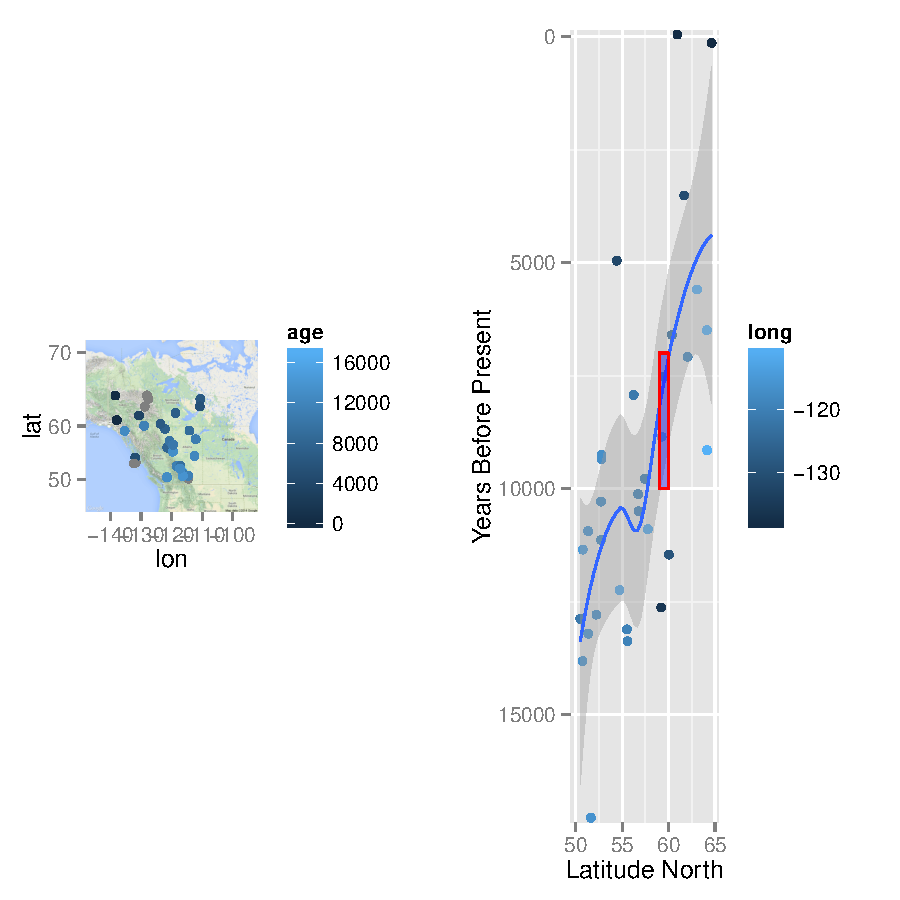
\includegraphics{neotoma_sweave-007}

And so we see a clear pattern of migration by \emph{Pinus} in northwestern North America.  These results match up broadly with the findings of Strong and Hills (2013) who suggest that \emph{Pinus} reached a northern extent between 59 and 60^oN at approximately 7 - 10kyr as a result of geographic barriers.

\end{document}
